\let\negmedspace\undefined
\let\negthickspace\undefined
\documentclass[journal]{IEEEtran}
\usepackage[a5paper, margin=10mm, onecolumn]{geometry}
\usepackage{tfrupee} 

\setlength{\headheight}{1cm} 
\setlength{\headsep}{0mm}     

\usepackage{gvv-book}
\usepackage{gvv}
\usepackage{cite}
\usepackage{amsmath,amssymb,amsfonts,amsthm}
\usepackage{algorithmic}
\usepackage{graphicx}
\usepackage{textcomp}
\usepackage{xcolor}
\usepackage{txfonts}
\usepackage{listings}
\usepackage{enumitem}
\usepackage{mathtools}
\usepackage{gensymb}
\usepackage{comment}
\usepackage[breaklinks=true]{hyperref}
\usepackage{tkz-euclide} 
\usepackage{listings}                                        
\def\inputGnumericTable{}                                 
\usepackage[latin1]{inputenc}                                
\usepackage{color}                                            
\usepackage{array}                                            
\usepackage{longtable}                                       
\usepackage{calc}                                             
\usepackage{multirow}                                         
\usepackage{hhline}                                           
\usepackage{ifthen}                                           
\usepackage{lscape}

\begin{document}

\bibliographystyle{IEEEtran}
\vspace{3cm}

\title{4.4.4}
\author{AI25BTECH11008 - Chiruvella Harshith Sharan}
{\let\newpage\relax\maketitle}

\renewcommand{\thefigure}{\theenumi}
\renewcommand{\thetable}{\theenumi}
\setlength{\intextsep}{10pt} 

\numberwithin{equation}{enumi}
\numberwithin{figure}{enumi}
\renewcommand{\thetable}{\theenumi}

\textbf{Question}: A line passes through the point with position vector 
\[
\vec{A} = 2\hat{i} - \hat{j} + 4\hat{k}
\]
and is in the direction of the vector 
\[
\vec{d} = \hat{i} + \hat{j} - 2\hat{k}.
\] 
Find the equation of the line. \\\\[0.3cm]

\textbf{Solution}: \\\\[0.3cm]

The line passes through point 
\begin{equation}
\vec{A} = \myvec{2 \\ -1 \\ 4}
\end{equation}
and has direction vector 
\begin{equation}
\vec{d} = \myvec{1 \\ 1 \\ -2}.
\end{equation}

\vspace{0.3cm}

The vector equation of a line is
\begin{equation}
\vec{r} = \vec{A} + \lambda \vec{d}, \quad \lambda \in \mathbb{R}.
\end{equation}

Substituting the given values,
\begin{equation}
\vec{r} = \myvec{2 \\ -1 \\ 4} + \lambda \myvec{1 \\ 1 \\ -2}.
\end{equation}

\vspace{0.3cm}

Thus, the equation of the line is
\[
\vec{r} = \myvec{2 + \lambda \\ -1 + \lambda \\ 4 - 2\lambda}, \quad \lambda \in \mathbb{R}.
\]

\vspace{0.3cm}

Or equivalently, in symmetric form,
\[
\frac{x-2}{1} = \frac{y+1}{1} = \frac{z-4}{-2}.
\]

\begin{figure}[htbp]
    \centering
    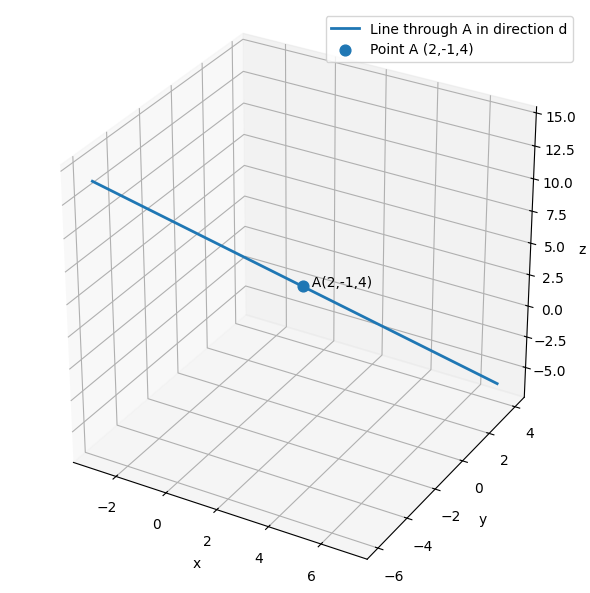
\includegraphics[width=0.8\linewidth]{figs/fig1.jpg}
    \caption{Graph showing the line through point $\vec{A}$ in direction $\vec{d}$}
    \label{fig:fig1}
\end{figure}

\end{document}
